% !TEX encoding = UTF-8 Unicode
%\documentclass[12pt,reqno]{amsart}
\documentclass{article}
%\usepackage{tocloft}

%\cftsetindents{section}{0.5in}{0.5in}
%\cftsetindents{subsection}{0.5in}{0.5in}
\usepackage[utf8]{inputenc}
%\usepackage[dvips]{graphicx,graphics}
\usepackage{listings}
\usepackage{xcolor}
\definecolor{dkgreen}{rgb}{0,0.6,0}
\definecolor{gray}{rgb}{0.4,0.4,0.4}
\usepackage{graphicx}
\usepackage{euscript}
\usepackage{graphics}
%\usepackage{russcorr}
\usepackage[active]{srcltx} % SRC Specials: DVI [Inverse] Search
\usepackage{amssymb,amsmath,amsthm,amsfonts}
\usepackage{amsopn}

\usepackage{verbatim}
\usepackage{hyperref}
\hypersetup{
    colorlinks,
    citecolor=black,
    filecolor=black,
    linkcolor=blue,
    urlcolor=blue
}
\usepackage{titlesec}
\titleformat{\section}[block]{\color{blue}\Large\bfseries\filcenter}{\thesection.}{1em}{}
\titleformat{\subsection}[hang]{\color{blue}\large\filcenter}{\thesubsection.}{1em}{}

\usepackage{a4wide}
\lstset{language=C++,
                basicstyle=\ttfamily,
		frame=tb,
		  aboveskip=3mm,
		  belowskip=3mm,
		  numberstyle=\tiny\color{gray},
		  keywordstyle=\color{blue},
		  commentstyle=\color{dkgreen},
		  stringstyle=\color{mauve},
		  breaklines=true,
		  breakatwhitespace=true,
		  tabsize=3,
                morecomment=[l][\color{magenta}]{\#}
}
\begin{document}

\begin{center}
 \Large{\bf RAST: highly distributed DB project.}

{\large {\bf Produced by NOA team}}
\end{center}

\tableofcontents

\newpage
\section{Algorithmic basis}

\subsection{Free-list multi-level allocator}

On of the most important steps in order to make a low-latency system is to consider the allocation problem. The problem is that sometimes different components of the program require very small parts of memory to be allocated. Asking the system to allocate memory directly can result in slower performance. That's why it is better to allocate large memory segment and distribute its parts among several consumers.

But here we face another difficulty, so called fragmentation problem. Imagine that an allocated segment is separated into several parts owned by consumers. Some time after, some of the consumers returned their own parts to allocator (calling deallocate method). Afterwards it appears that the returned memory in control of allocator is represented as distinct small fragments. Those fragments cannot be given to a consumer, who asks for a larger memory segment, than the size of the separate fragment. If there is a lot of such unusable fragments, we would have a lot of memory allocated, which will never be used. In order to avoid this problem, we have to force each small fragment to be used by a consumer who asks for a small amount of memory.

The main idea is to use a memory levels.

\begin{center}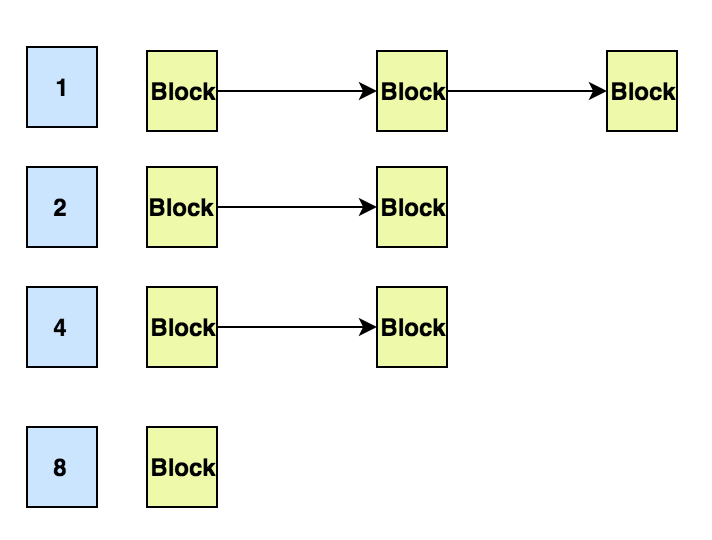
\includegraphics[width=0.5 \textwidth]{image1.png}\end{center}

For each block size we calculate an integer part of $log(size)$ and put all blocks of memory in the corresponding list.

By means of the list, we can easily find the block of needed size and remove (detach) it from the list, giving ownership to the consumer, who asked to allocate memory. Likewise, when a consumer asks to deallocate the block, we may put (attach) it again in the list.

Also we want to join small segments of memory returned by consumers to one large segment in case if they go one after another in the global memory space. In order to do this, let us have the following structure of the memory block:

\begin{center}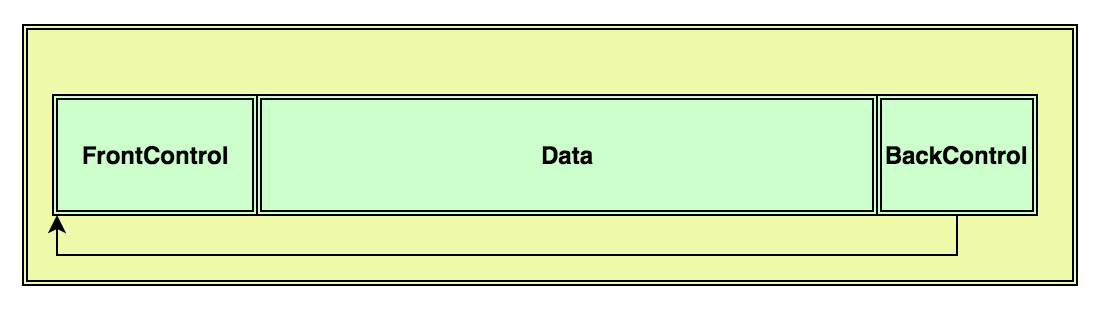
\includegraphics[width=0.5 \textwidth]{image2.png}\end{center}

The block will consist of three logical parts:

$\bullet$ FrontControl, which stores the $data\_size$ which is size of the block, $localnext$ and $localprev$ pointers, $offset$ in external allocated segment, and $total\_size$ of external segment, and $is\_owned$ -- whether the block is owned by the allocator itself or was it given away to the consumer.

$\bullet$ Data -- raw byte space, which would be given an external consumer to control

$\bullet$ BackControl, which stores pointer to the FrontControl (pointer to the beginning of the entire block)

$localprev$ and $localnext$ pointers will help us to build freelists, which were described above. BackControl block will help us to find the block, previous to some specific Block, so that we could join two blocks together in case they both have been returned to the allocator. Here is how joining procedure works:

\begin{center}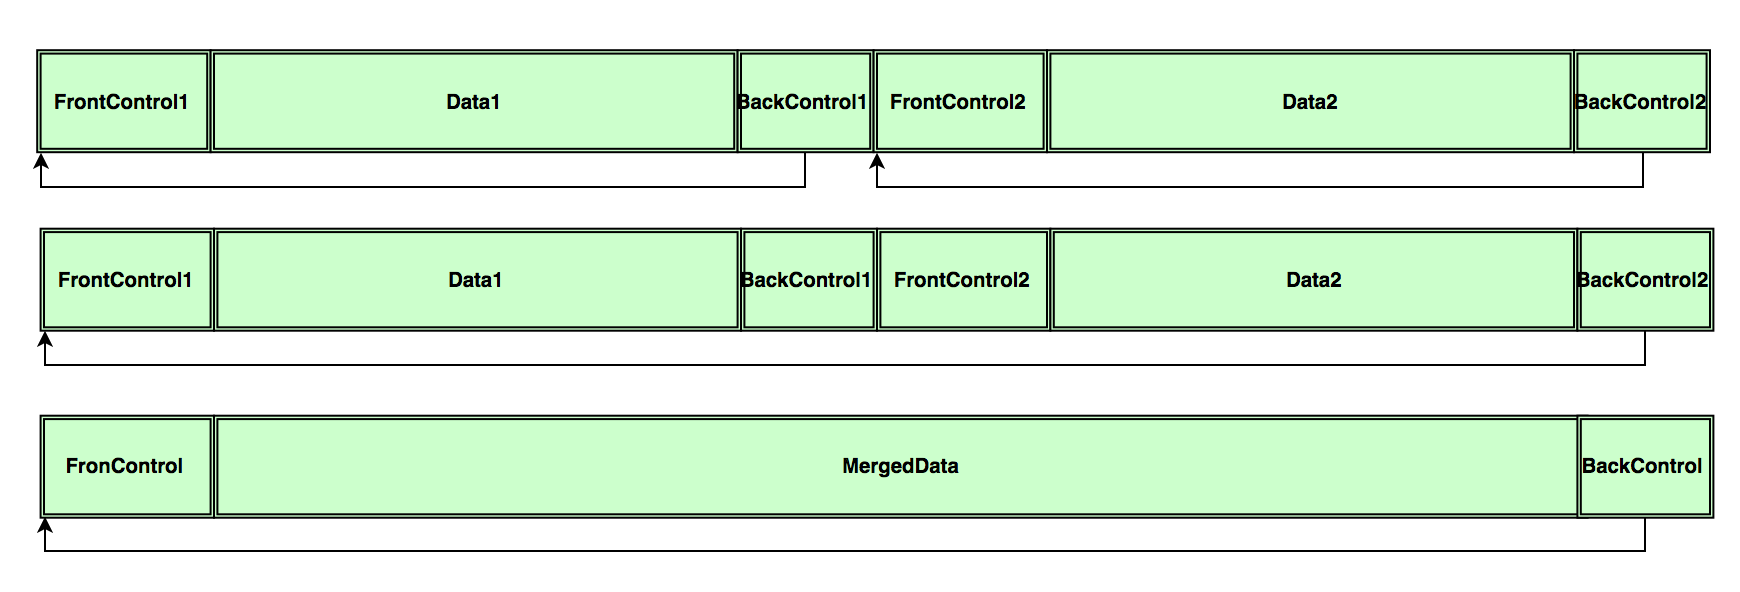
\includegraphics[width=1 \textwidth]{image3.png}\end{center}

The steps are very simple:

$\bullet$ detach first block from its list

$\bullet$ detach second block from its list

$\bullet$ point BackControl2 to FrontControl1

$\bullet$ change FrontControl1 information about block size

$\bullet$ do nothing about BackControl1 and FrontControl2, because now we threat them as a garbage part of MergedData, and we do not have to care about their contents so far

$\bullet$ attach new merged block to its new list (based on $log(size)$ where $size$ is a sum of sizes of these two blocks) by changing $localprev$ and $localnext$ pointers of FrontControl.

\smallskip

Also, one can easily imagine how to split one large block into two smaller.

\smallskip

Blocks contained in the same external memory segment (which allocator asked from the system) may be joined and split so that we know exactly how many consequent free to use bytespace fragments do we have.
\smallskip

Finally, the allocation procedure is the following:

$\bullet$ calculate integral part $N = int(log(size))$ of the size of the memory consumer asks to allocate

$\bullet$ if the corresponding $N$-th list of blocks is empty, we allocate several external blocks of the sizes $2^{N}$ and build Block structure upon each of them, putting blocks to the $N$-th list

$\bullet$ detach first block from the list

$\bullet$ split the block into two blocks: first block has exactly needed size, second block consists of what is remained

$\bullet$ attach second block to its corresponding list

$\bullet$ mark the first block as not owned by allocator

$\bullet$ return a pointer to the Data section of the first block to a consumer

\smallskip

The deallocation procedure:

$\bullet$ receive from a consumer a pointer to deallocate data

$\bullet$ calculate the pointer to FrontControl (by subtracting $sizeof(FrontControl)$ from Data pointer)

$\bullet$ mark block as owned by the allocator

$\bullet$ read $offset$ from FrontControl, if $offset > 0$, than there is some previous block in the external memory segment.

$\bullet$ calculate the pointer to BackControl of the previous block (by subtracting $sizeof(BackControl)$ from the pointer to the current block)

$\bullet$ get the pointer to the FrontControl of the previous block via BackControl

$\bullet$ check whether the previous block is owned by the allocator and if it is, merge it with the current block

$\bullet$ if $offset < total\_size$ where $total\_size$ is the size of external allocated memory segment, we may want to check whether we can merge with the forthcoming block

$\bullet$ calculate the pointer to the FrontControl of the forthcoming block (by adding $data\_size + sizeof(FrontControl) + sizeof(BackControl)$ to the pointer to the current block)

$\bullet$ check if the forthcoming block is owned by allocator using its FrontControl and if it is, merge it with the current block.

\newpage

\section{Detailed Code Architecture (classes and methods)}

\subsection{Lock-free queue}

$LockFreeQueue<TElement>$ is obviously an implementation of lock-free queue. It contains the following functions:


\begin{lstlisting}
LockFreeQueue<TElement> {
	void Push(TElement new_element);
	// Exceptions:
	// 	Strong exception safety: in case of failure
	// 	the element is not pushed to the queue,
	// 	there are no visible side effects

	std::unqiue_ptr<TElement> Pop() noexcept;
	// Return value:
	// 	nullptr unique_ptr if the queue was empty,
	// 	unique_ptr pointing on TElement in case of successful pop
};
\end{lstlisting}

\end{document}

